\documentclass{beamer}
\usetheme{metropolis}
\usepackage{graphicx}
\usepackage{subfig}
\usepackage{tcolorbox}
\title{Algebra-Based Physics-2: Electricity, Magnetism, and Modern Physics (PHYS135B-01): Unit 4}
\author{Jordan Hanson}
\institute{Whittier College Department of Physics and Astronomy}

\begin{document}
\maketitle

\section{Unit 2 Review}

\begin{frame}{Unit 2 Summary}
\textbf{Reading: Chapters 20 and 21}
\begin{enumerate}
\item Current, Ohm's Law, resistors and conductors
\item DC circuits I
\item Nerve signals
\item \alert{DC circuits II}
\end{enumerate}
\end{frame}

\section{Unit 2 Review Problems}

\begin{frame}{Unit 2 Review Problems}
Consider a proton with mass $m$ and charge $q_{\rm p}$.  The proton is located in a region with electric field $E$, and it has initial velocity $v_{\rm i}$ at time $t = 0$.  What is the acceleration of the proton?  What is the proton velocity $v_{\rm f}$ after a time $t$?
\begin{itemize}
\item A: $a = \frac{m}{q_{\rm p}} E$, $v_{\rm f}=v_{\rm i}+t$
\item B: $a = \frac{m}{q_{\rm p}} E$, $v_{\rm f}=v_{\rm i}+\frac{m}{q_{\rm p}} E t$
\item C: $a = \frac{q_{\rm p}}{m} E$, $v_{\rm f}=v_{\rm i}+\frac{q_{\rm p}}{m} E t$
\item D: $a = \frac{q_{\rm p}}{m} E$, $v_{\rm f}=v_{\rm i}+t$
\end{itemize}
\end{frame}

\begin{frame}{Unit 2 Review Problems}
Consider a line of charge with linear charge density $\lambda$ C/m, aligned with the z-axis.  What is most likely the expression for the electric field a distance $r$ away from the line?  In this coordinate system, $\phi$ is the angle measured counter-clockwise from the x-axis in the x-y plane, and $z$ is the height above the x-y plane. \textit{Hint: think about symmetry of the charge distribution.}
\begin{itemize}
\item A: $\frac{2k\lambda}{r} \hat{r}$
\item B: $\frac{2k\lambda}{r^2} \hat{r}$
\item C: $\frac{2k\lambda}{r} \cos\phi \hat{r}$
\item D: $\frac{2k\lambda}{r} \sin\phi \hat{r}$
\end{itemize}
\end{frame}

\begin{frame}{Unit 2 Review Problems}
Consider a 12V battery driving current through a system with a total resistance of $1$ k$\Omega$.  What is the current?  What is the power consumption? 
\begin{itemize}
\item A: 12 mA, 144 W
\item B: 144 mA, 12 mW
\item C: 12 mA, 144 mW
\item D: 14.4 A, 144 W
\end{itemize}
\end{frame}

\section{Summary}

\begin{frame}{Unit 2 Summary}
\textbf{Reading: Chapter 22}
\begin{enumerate}
\item Magnets and magnetic fields
\item Force on a moving charge in a magnetic field
\item \textbf{The Hall effect}
\item Magnetic forces on conductors
\item \alert{Amp\`{e}re's Law}
\end{enumerate}
\end{frame}

\section{JITT - Reading Quiz Results}

\begin{frame}{JITT 1.5}
\begin{enumerate}
\item List the ways in which magnetic field lines and electric field lines are similar. For example, the field direction is tangent to the line at any point in space. Also list the ways in which they differ.
\item Is the Earth’s magnetic field parallel to the ground at all locations? If not, where is it parallel to the surface? Is its strength the same at all locations? If not, where is it greatest?
\item How is the Hall effect used to obtain information on the sign of the free charges in a conductor?
\end{enumerate}
\end{frame}

\begin{frame}{JITT 1.5}
\small
\textbf{List the ways in which magnetic field lines and electric field lines are similar. For example, the field direction is tangent to the line at any point in space. Also list the ways in which they differ.} \\ \vspace{0.5cm}
``They are both vector field, but the electric field lines are more like rays while the magnetic field lines are closed loops.'' \\ \vspace{0.5cm}
``Magnetic field lines and electric field lines are similar because they never cross each other, the strength of the field is proportional to the number and closeness of field lines, and the field is unique at each point in space. However, they differ because the electric force is parallel to the field lines whereas magnetic force is perpendicular to the field lines.'' \\ \vspace{0.5cm}
``...Magnetic field lines are continuous, while electric field lines have starting and ending points.''
\end{frame}

\begin{frame}{JITT 1.5}
\small
\textbf{Is the Earth’s magnetic field parallel to the ground at all locations? If not, where is it parallel to the surface? Is its strength the same at all locations? If not, where is it greatest?} \\ \vspace{0.5cm}
``No it is not parallel to the ground at all locations. It is parallel to the surface at/near the equator. Its strength is no the same at all locations and is the greatest at the poles.'' \\ \vspace{0.5cm}
``Earth’s magnetic field is not parallel to the ground at all locations. The magnetic field is most commonly parallel in locations near the equator. Strength is not the same in all locations either. The magnetic south and north poles have the largest strength.'' \\ \vspace{0.5cm}
``The earth's magnetic field is not always parallel to the surface of the earth and may be perpendicular. The general trend is that the field is strongest near the magnetic poles and is weakest near the equator.''
\end{frame}

\begin{frame}{JITT 1.5}
\small
\textbf{How is the Hall effect used to obtain information on the sign of the free charges in a conductor?} \\ \vspace{0.5cm}
``Moving electrons feel a magnetic force toward one side of the conductor, leaving a net positive charge on the other side. This separation of charge creates a voltage. If electrons move to the left then the voltage is positive. If electrons move to the right voltage is negative.'' \\ \vspace{0.5cm}
``The Hall effect is the creation of voltage $\epsilon$, known as the Hall emf, across a current-carrying conductor by a magnetic field. The Hall emf is given by $\epsilon = Blv$ (B, v, and l, mutually perpendicular) for a conductor of width l through which charges move at a speed v . We can use this information to determine if the charges in a given conductor are positively or negatively charged.''
\end{frame}

\section{Magnets and magnetic fields}

\begin{frame}{Magnets and magnetic fields}
What is a cross-product and how does it work? \\ \vspace{0.25cm}
\begin{figure}
\centering
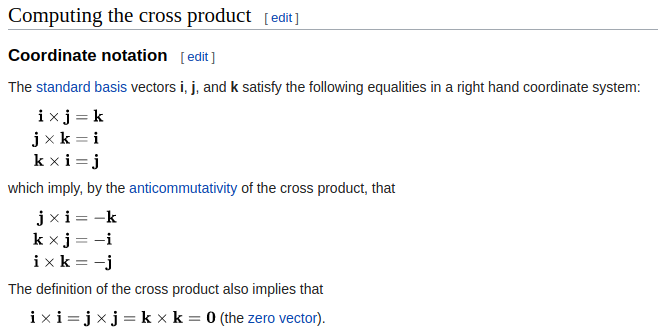
\includegraphics[width=0.75\textwidth]{figures/crossP.png}
\caption{\label{fig:crossP} The cross-product is a way of multiplying unit vectors.}
\end{figure}
\end{frame}

\begin{frame}{Magnets and magnetic fields}
Let $\vec{v} = 2\hat{i}$ and $w = -2 \hat{j}$.  What is $\vec{v} \times \vec{w}$?
\begin{itemize}
\item A: $-4 \hat{k}$
\item B: $4 \hat{k}$
\item C: $-2 \hat{i}$
\item D: $2 \hat{j}$
\end{itemize}
\end{frame}

\begin{frame}{Magnets and magnetic fields}
Let $\vec{v} = 3\hat{j}$ and $w = 5 \hat{k}$.  What is $\vec{v} \times \vec{w}$?
\begin{itemize}
\item A: $15 \hat{i}$
\item B: $5 \hat{j}$
\item C: $3 \hat{i}$
\item D: $15 \hat{k}$
\end{itemize}
\end{frame}

\begin{frame}{Magnets and magnetic fields}
Let $\vec{v} = 3\hat{i} \times 3\hat{j}$ and $w = 2 \hat{k}$.  What is $\vec{v} \times \vec{w}$?
\begin{itemize}
\item A: $-6 \hat{j} + 6\hat{k}$
\item B: $-6 \hat{j} + 6\hat{i}$
\item C: $6 \hat{j} + 6\hat{i}$
\item D: $6 \hat{k} + 6\hat{i}$
\end{itemize}
\end{frame}

\begin{frame}{Magnets and magnetic fields}
\textbf{Group board exercise:} Compute the following cross product:
\begin{align}
\vec{v} &= 2\hat{i}-2\hat{j} \\
\vec{w} &= 4\hat{j}-4\hat{i} \\
\vec{v} \times \vec{w} &= ??
\end{align}
\end{frame}

\begin{frame}{Magnets and magnetic fields}
\textbf{Group board exercise:} Compute the following cross product:
\begin{align}
\vec{v} &= 2\hat{i}-2\hat{j}+\hat{k} \\
\vec{w} &= 4\hat{j}-4\hat{i}-\hat{k} \\
\vec{v} \times \vec{w} &= ??
\end{align}
\end{frame}

\begin{frame}{Magnets and magnetic fields}
\begin{tcolorbox}[colback=white,colframe=red!40!blue,title=The Lorentz Force]
\alert{Let a particle with charge $q$ and velocity $\vec{v}$ move through a \textit{magnetic field} $\vec{B}$.  The \textbf{Lorentz force} on the charged particle is
\begin{equation}
\vec{F}_{\rm L} = q\vec{v} \times \vec{B}
\label{eq:Lorentz}
\end{equation}}
\end{tcolorbox}
\textit{As a helpful memory tool, we have the right-hand rule to remember the direction of the cross-product.}  \textbf{The units of the magnetic field are the Telsa}, after Nikola Tesla.  We also have the Gauss which is $10^{-4}$ Tesla.
\end{frame}

\begin{frame}{Magnets and magnetic fields}
\begin{figure}
\centering
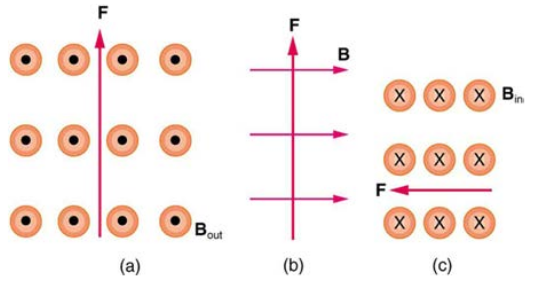
\includegraphics[width=0.75\textwidth]{figures/lorentzProblem.png}
\caption{\label{fig:lorentzProblem} Three different magnetic field and charge scenarios.  The vector $\vec{F}$ is the direction of the Lorentz force, and the magnetic field is uniform.  A dot indicates that the magnetic field is coming out of the page, and an x indicates that the field is going into the page.}
\end{figure}
\end{frame}

\begin{frame}{Magnets and magnetic fields}
\begin{columns}[T]
\begin{column}{0.3\textwidth}
In which of the diagrams is a positively charged particle moving to the left?
\begin{itemize}
\item A: A
\item B: B
\item C: C
\item D: WAT WAT WAT
\end{itemize}
\end{column}
\begin{column}{0.7\textwidth}
\begin{figure}
\centering
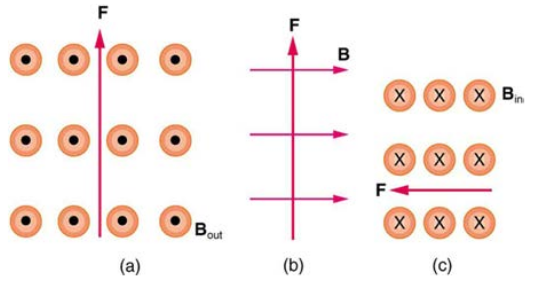
\includegraphics[width=0.75\textwidth]{figures/lorentzProblem.png}
\caption{\label{fig:lorentzProblem2} Three different magnetic field and charge scenarios.}
\end{figure}
\end{column}
\end{columns}
\end{frame}

\begin{frame}{Magnets and magnetic fields}
\begin{columns}[T]
\begin{column}{0.3\textwidth}
In which of the diagrams is a positively charged particle moving upwards?
\begin{itemize}
\item A: A
\item B: B
\item C: C
\item D: WAT WAT WAT
\end{itemize}
\end{column}
\begin{column}{0.7\textwidth}
\begin{figure}
\centering
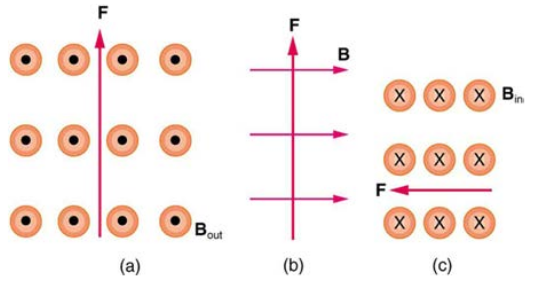
\includegraphics[width=0.75\textwidth]{figures/lorentzProblem.png}
\caption{\label{fig:lorentzProblem3} Three different magnetic field and charge scenarios.}
\end{figure}
\end{column}
\end{columns}
\end{frame}

\begin{frame}{Magnets and magnetic fields}
\begin{columns}[T]
\begin{column}{0.3\textwidth}
In which of the diagrams is a negatively charged particle into the page?
\begin{itemize}
\item A: A
\item B: B
\item C: C
\item D: WAT WAT WAT
\end{itemize}
\end{column}
\begin{column}{0.7\textwidth}
\begin{figure}
\centering
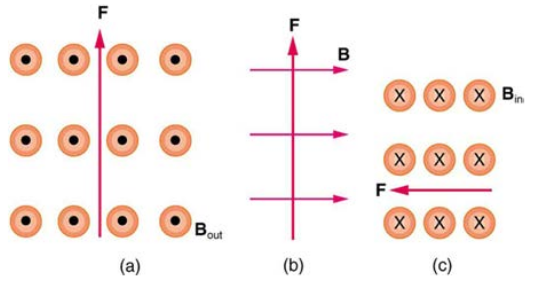
\includegraphics[width=0.75\textwidth]{figures/lorentzProblem.png}
\caption{\label{fig:lorentzProblem4} Three different magnetic field and charge scenarios.}
\end{figure}
\end{column}
\end{columns}
\end{frame}

\begin{frame}{Magnets and magnetic fields}
\begin{columns}[T]
\begin{column}{0.3\textwidth}
In which of the diagrams is a negatively charged particle to the right?
\begin{itemize}
\item A: A
\item B: B
\item C: C
\item D: WAT WAT WAT
\end{itemize}
\end{column}
\begin{column}{0.7\textwidth}
\begin{figure}
\centering
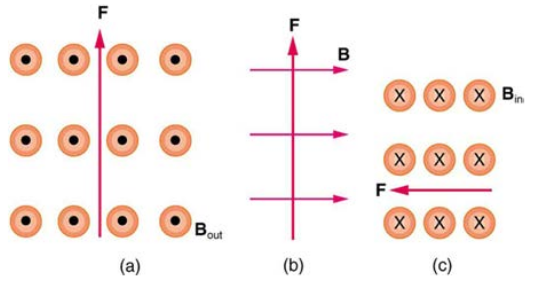
\includegraphics[width=0.75\textwidth]{figures/lorentzProblem.png}
\caption{\label{fig:lorentzProblem5} Three different magnetic field and charge scenarios.}
\end{figure}
\end{column}
\end{columns}
\end{frame}

\begin{frame}{Magnets and magnetic fields}
A theorem for the magnitude of the cross-product:  Let $\vec{a}$ and $\vec{b}$ be vectors and $\theta$ be the angle between them.  The magnitude of the cross-product is
\begin{equation}
|\vec{a} \times \vec{b}| =  a b \sin\theta
\end{equation}
Thus, the magnitude of the Lorentz force is
\begin{equation}
F_{\rm L} = q v B \sin\theta
\end{equation}
The angle $\theta$ is between the velocity and the magnetic field.
\end{frame}

\begin{frame}{Magnets and magnetic fields}
A cosmic ray proton moving toward the Earth at $3 \times 10^{6}$ m/s experiences a magnetic force of $2 \times 10^{-17}$ N. What is the strength of the magnetic field if there is a $45$ degree angle between it and the proton’s velocity?  (Remember that $q$ for a proton is $1.6 \times 10^{-19}$ C).
\begin{itemize}
\item A: 0.1 Gauss
\item B: 0.6 Gauss
\item C: 1 Gauss
\item D: 6 Gauss
\end{itemize}
\end{frame}

\begin{frame}{Magnets and magnetic fields}
\begin{figure}
\centering
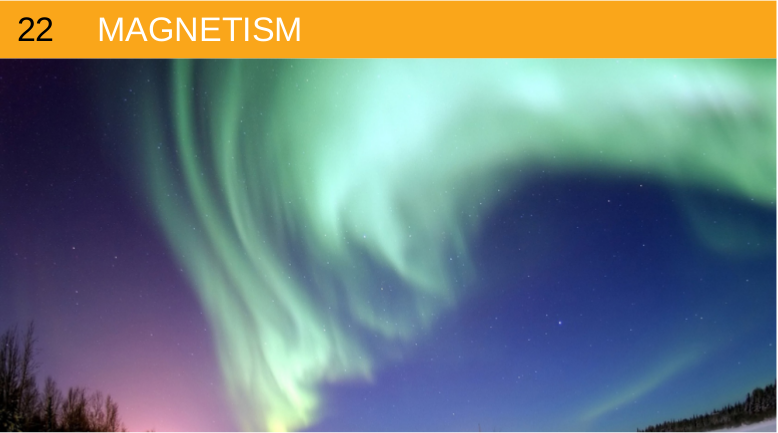
\includegraphics[width=0.9\textwidth]{figures/aurora.png}
\caption{\label{fig:aurora} The aurora borealis, or northern lights.}
\end{figure}
\end{frame}

\begin{frame}{Magnets and magnetic fields}
A cool talk on the aurora borealis:
\url{https://youtu.be/czMh3BnHFHQ} \\
\begin{figure}
\centering
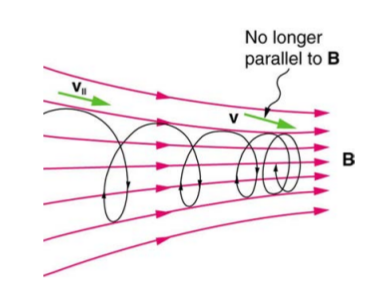
\includegraphics[width=0.45\textwidth]{figures/mag1.png}
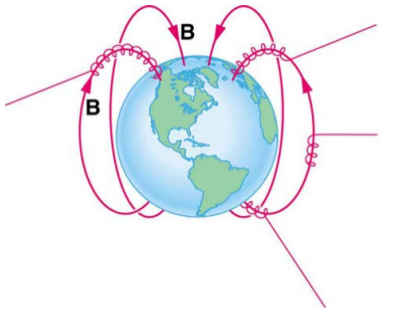
\includegraphics[width=0.45\textwidth]{figures/mag2.png}
\end{figure}
One un-explained piece: what does it mean for the electrons and protons to \textit{high-five} the neutral oxygen and nitrogen atoms?
\end{frame}

\section{The Hall Effect}

\begin{frame}{The Hall Effect}
\begin{figure}
\centering
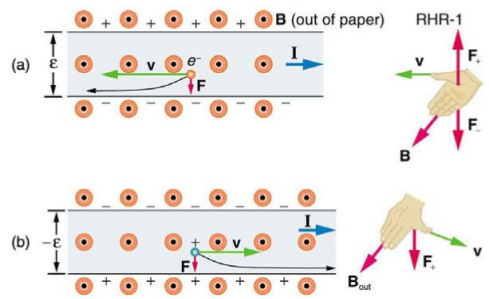
\includegraphics[width=0.6\textwidth]{figures/hall.png}
\caption{\label{fig:hall} Diagram of the Hall effect.  The Hall emf reveals the sign of the moving charges.}
\end{figure}
The Hall emf is 
\begin{equation}
\epsilon = Blv
\end{equation}
The $B$ is the magnetic field, $l$ is the length across the region where charge is flowing, and $v$ is the velocity of the charges.
\end{frame}

\begin{frame}{The Hall Effect}
\textbf{Group board exercise:} Let $n$ be the charge number density in a conductor.  Let $q$ be the charge of an electron.  Let $A$ be the cross-sectional area, and $I$ be the current.  Recall that the \textit{drift velocity of charges in a wire} is given by the equation
\begin{equation}
v_d = \frac{I}{nqA}
\end{equation}
The Hall emf is $\epsilon = Blv$.  Let $v = v_d$, and substitute the first equation into the second equation, and solve for $n$.  Choose reasonable numbers for the current, diameter of a metal wire, and assume a uniform 0.001 T magnetic field is being created around the wire.  Assume a drift velocity of about 1 mm/sec, and solve for $n$.
\end{frame}

\section{Conclusion}

\begin{frame}{Unit 2 Summary}
\textbf{Reading: Chapter 22}
\begin{enumerate}
\item Magnets and magnetic fields
\item Force on a moving charge in a magnetic field
\item \textbf{The Hall effect}
\item Magnetic forces on conductors
\item \alert{Amp\`{e}re's Law}
\end{enumerate}
\end{frame}

\section{Answers}

\begin{frame}{Answers}
\tiny
\begin{columns}[T]
\begin{column}{0.5\textwidth}
\begin{itemize}
\item $a = \frac{q_{\rm p}}{m} E$, $v_{\rm f}=v_{\rm i}+\frac{q_{\rm p}}{m} E t$
\item $\frac{2k\lambda}{r} \hat{r}$
\item 12 mA, 144 mW
\item $-4 \hat{k}$
\item $15 \hat{i}$
\item $-6 \hat{j}+6\hat{i}$
\item A
\item C
\item B
\item A
\item 0.6 Gauss
\end{itemize}
\end{column}
\begin{column}{0.5\textwidth}
\begin{itemize}
\item 
\end{itemize}
\end{column}
\end{columns}
\end{frame}

\end{document}
